\documentclass[17pt,mathserif]{beamer}
\usepackage{pdfrender}
\usepackage{tikz}
\usepackage{times}
\usepackage{caption}
\usepackage{subcaption}
\usepackage{ifthen}
%\usepackage[backend=bibtex]{biblatex}
\usepackage[style=authortitle,backend=bibtex]{biblatex}

\usetikzlibrary{shapes,arrows,mindmap,backgrounds}
\usepackage{default}





\usetikzlibrary{decorations.pathmorphing} % noisy shapes
\usetikzlibrary{fit}					% fitting shapes to coordinates
\usetikzlibrary{backgrounds}	% drawing the background after the foreground
\usetikzlibrary{fadings}
\usetikzlibrary{arrows}

\tikzset{
    rectangle with rounded corners north west/.initial=4pt,
    rectangle with rounded corners south west/.initial=4pt,
    rectangle with rounded corners north east/.initial=4pt,
    rectangle with rounded corners south east/.initial=4pt,
}
\makeatletter
\pgfdeclareshape{rectangle with rounded corners}{
    \inheritanchorborder[from=rectangle]
    \savedmacro{\neoffset}{
        \pgfkeysgetvalue{/tikz/rectangle with rounded corners north east}{\pgf@rectc}
        \let\neoffset\pgf@rectc
    }
    \savedmacro{\nwoffset}{
        \pgfkeysgetvalue{/tikz/rectangle with rounded corners north west}{\pgf@rectc}
        \let\nwoffset\pgf@rectc
    }
    \savedmacro{\seoffset}{
        \pgfkeysgetvalue{/tikz/rectangle with rounded corners south east}{\pgf@rectc}
        \let\seoffset\pgf@rectc
    }
    \savedmacro{\swoffset}{
        \pgfkeysgetvalue{/tikz/rectangle with rounded corners south west}{\pgf@rectc}
        \let\swoffset\pgf@rectc
    }
    \savedanchor{\north}{
        \pgf@y=.5\ht\pgfnodeparttextbox
        \pgf@x=0pt
        \setlength{\pgf@ya}{\pgfshapeminheight}
        \ifdim\pgf@y<.5\pgf@ya
        \pgf@y=.5\pgf@ya
        \fi
    }
    \savedanchor{\south}{
        \pgf@y=-.5\ht\pgfnodeparttextbox
        \pgf@x=0pt
        \setlength{\pgf@ya}{\pgfshapeminheight}
        \ifdim\pgf@y>-.5\pgf@ya
        \pgf@y=-.5\pgf@ya
        \fi
    }
    \savedanchor{\east}{
        \pgf@y=0pt
        \pgf@x=.5\wd\pgfnodeparttextbox
        \addtolength{\pgf@x}{2ex}
        \setlength{\pgf@xa}{\pgfshapeminwidth}
        \ifdim\pgf@x<.5\pgf@xa
        \pgf@x=.5\pgf@xa
        \fi
    }
    \savedanchor{\west}{
        \pgf@y=0pt
        \pgf@x=-.5\wd\pgfnodeparttextbox
        \addtolength{\pgf@x}{-2ex}
        \setlength{\pgf@xa}{\pgfshapeminwidth}
        \ifdim\pgf@x>-.5\pgf@xa
        \pgf@x=-.5\pgf@xa
        \fi
    }
    \savedanchor{\northeast}{
        \pgf@y=.5\ht\pgfnodeparttextbox % height of the box
        \pgf@x=.5\wd\pgfnodeparttextbox % width of the box
        \addtolength{\pgf@x}{2ex}
        \setlength{\pgf@xa}{\pgfshapeminwidth}
        \ifdim\pgf@x<.5\pgf@xa
        \pgf@x=.5\pgf@xa
        \fi
        \setlength{\pgf@ya}{\pgfshapeminheight}
        \ifdim\pgf@y<.5\pgf@ya
        \pgf@y=.5\pgf@ya
        \fi
    }
    \savedanchor{\southwest}{
        \pgf@y=-.5\ht\pgfnodeparttextbox
        \pgf@x=-.5\wd\pgfnodeparttextbox
        \addtolength{\pgf@x}{-2ex}
        %     \pgf@x=0pt
        \setlength{\pgf@xa}{\pgfshapeminwidth}
        \ifdim\pgf@x>-.5\pgf@xa
        \pgf@x=-.5\pgf@xa
        \fi
        \setlength{\pgf@ya}{\pgfshapeminheight}
        \ifdim\pgf@y>-.5\pgf@ya
        \pgf@y=-.5\pgf@ya
        \fi
    }
    \anchor{text}{%
        \northeast%
        \pgf@x=-.5\wd\pgfnodeparttextbox%
        \pgfmathsetlength{\pgf@y}{-.5ex}
    }
    \anchor{north east}{
        \northeast
        \pgfmathsetmacro{\nw}{(1-sin(45))*\neoffset}
        \addtolength{\pgf@x}{-\nw pt}
        \addtolength{\pgf@y}{-\nw pt}
    }
    \anchor{center}{
        \pgf@x=0pt
        \pgf@y=0pt
    }
    \anchor{south west}{
        \southwest
        \pgfmathsetmacro{\nw}{(1-sin(45))*\swoffset}
        \addtolength{\pgf@x}{\nw pt}
        \addtolength{\pgf@y}{\nw pt}
    }
    \anchor{north west}{
        \northeast
        \pgfmathsetmacro{\temp@x}{\pgf@x}
        \southwest
        \pgfmathsetmacro{\temp@xtwo}{\pgf@x}
        \northeast
        \pgfmathsetmacro{\xdiff}{\temp@x-\temp@xtwo}
        \def\pgf@xa{\pgf@x-\xdiff}
        \
        \pgfmathsetmacro{\nw}{(1-sin(45))*\nwoffset}
        \def\pgf@xaa{\pgf@xa+\nw}
        \def\pgf@yaa{\pgf@y-\nw}
        \pgfpoint{\pgf@xaa}{\pgf@yaa}
    }
    \anchor{south east}{
        \southwest
        \pgfmathsetmacro{\temp@x}{\pgf@x}
        \northeast
        \pgfmathsetmacro{\temp@xtwo}{\pgf@x}
        \southwest
        \pgfmathsetmacro{\xdiff}{\temp@x-\temp@xtwo}
        \def\pgf@xa{\pgf@x-\xdiff}
        \pgfmathsetmacro{\nw}{(1-sin(45))*\seoffset}
        \def\pgf@xaa{\pgf@xa-\nw}
        \def\pgf@yaa{\pgf@y+\nw}
        \pgfpoint{\pgf@xaa}{\pgf@yaa}
    }
    \anchor{south}{\south}
    \anchor{north}{\north}
    \anchor{east}{\east}
    \anchor{west}{\west}
    \backgroundpath{% this is new
        % store lower right in xa/ya and upper right in xb/yb
        \southwest \pgf@xa=\pgf@x \pgf@ya=\pgf@y
        \northeast \pgf@xb=\pgf@x \pgf@yb=\pgf@y
        % construct main path
        \pgfkeysgetvalue{/tikz/rectangle with rounded corners north west}{\pgf@rectc}
        \pgfsetcornersarced{\pgfpoint{\pgf@rectc}{\pgf@rectc}}
        \pgfpathmoveto{\pgfpoint{\pgf@xa}{\pgf@ya}}
        \pgfpathlineto{\pgfpoint{\pgf@xa}{\pgf@yb}}
        \pgfkeysgetvalue{/tikz/rectangle with rounded corners north east}{\pgf@rectc}
        \pgfsetcornersarced{\pgfpoint{\pgf@rectc}{\pgf@rectc}}
        \pgfpathlineto{\pgfpoint{\pgf@xb}{\pgf@yb}}
        \pgfkeysgetvalue{/tikz/rectangle with rounded corners south east}{\pgf@rectc}
        \pgfsetcornersarced{\pgfpoint{\pgf@rectc}{\pgf@rectc}}
        \pgfpathlineto{\pgfpoint{\pgf@xb}{\pgf@ya}}
        \pgfkeysgetvalue{/tikz/rectangle with rounded corners south west}{\pgf@rectc}
        \pgfsetcornersarced{\pgfpoint{\pgf@rectc}{\pgf@rectc}}
        \pgfpathclose
    }
}
\makeatother


\pgfdeclareradialshading{oncentre}{\pgfpoint{0cm}{0cm}}%
    {color(0cm)=(black!0);
    color(0.1cm)=(black!0);
    color(0.2cm)=(black!20);
    color(0.3cm)=(black!100);
    color(1cm)=(black!100);
    color(10cm)=(black!100!black)}

\pgfdeclareradialshading{offcentre}{\pgfpoint{0cm}{0cm}}%
    {color(0cm)=(black!100);
    color(0.1cm)=(black!100);
    color(0.2cm)=(black!80);
    color(0.3cm)=(black!60);
    color(0.4cm)=(black!45);
    color(0.45cm)=(black!30);
    color(1cm)=(black!0!white)}

\begin{document}
  \begin{frame}{This is the second slide}
\vspace*{-3em}
\hspace*{2em}
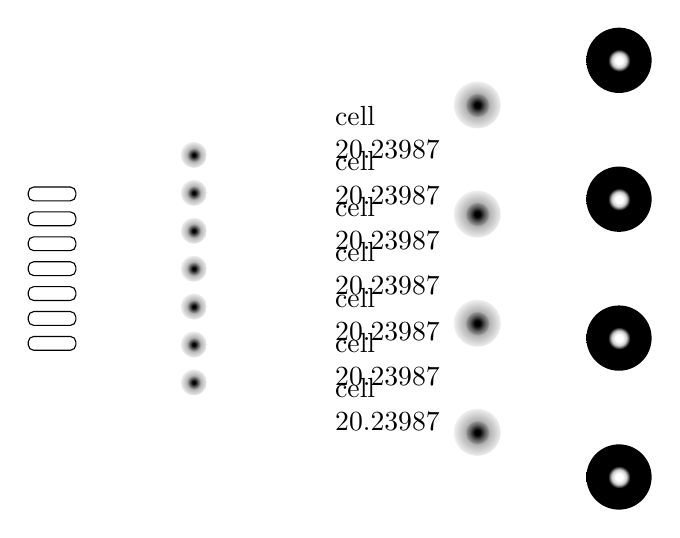
\begin{tikzpicture}[scale=0.9,
declare function={ radius(\x) = \x*\x*0.006em;
				   radiusLarge(\x) = \x*\x*0.1em;
				   nameMidget(\x,\y) = int(\x + 10*\y);
				   nameParasol(\x,\y) = int(\x + 20*\y);
                 },
]
\begin{scope}
    \foreach \y in {1,2,3,4,5,6,7} {
        \node[
            draw,
            shape=rectangle with rounded corners,
            minimum height=0.5em,
            minimum width=0.7em,
            rectangle with rounded corners north west=0.2em,
            rectangle with rounded corners south west=0.2em,
            rectangle with rounded corners north east=0.2em,
            rectangle with rounded corners south east=0.2em,
        ] at (0, -\y em) (receptor \y) {};
    }
\end{scope}
\begin{scope}[yshift=-4em, xshift=0em] 
            
    \foreach \x in {1,2,3,4} {
          \ifthenelse{\x < 3}
          {
            \foreach \y in {-1.5, -1,..., 1.5} {
                \pgfmathparse{Mod(\x,2)==1?1:0}

                \ifnum\pgfmathresult > 0
                	\pgfmathparse{(10*\y)}
                    \node[circle, shading=offcentre, text width=radius(\x),
                    minimum size=radius(\x)](cell \x \pgfmathresult ) at (2*\x, \y + \y*0.07*\x*\x )  {};
                \else
                	\pgfmathparse{(10*\y)}
                    \node[circle, text width=radius(\x),
                    minimum size=radius(\x)](cell \x \pgfmathresult) at (2*\x, \y + \y*0.07*\x*\x )  {cell \x \pgfmathresult};
                \fi
            }
          }{
            \foreach \y in {-1.5, -0.5,..., 1.5} {
                \pgfmathparse{Mod(\x,2)==1?1:0}
                \ifnum\pgfmathresult > 0
	                \pgfmathparse{(20*\y)}
                    \node[circle, shading=offcentre, text width=radiusLarge(\x),
                    minimum size=radiusLarge(\x)](cell \x \pgfmathresult) at (2*\x, \y + \y*0.06*\x*\x )  {};
                \else
					\pgfmathparse{(20*\y)}
                    \node[circle, shading=oncentre, text width=radiusLarge(\x),
                    minimum size=radiusLarge(\x)](cell \x \pgfmathresult) at (2*\x, \y + \y*0.06*\x*\x ) {};
                \fi
            }
          }
    }
%\end{scope}
%
%\begin{scope}
%\draw[bend right, ->]  (receptor 1) -- (cell1-15);
%    \foreach \r in {1,2,3,4,5,6,7} {
%        \foreach \x in {1,2,3,4} {
%            \foreach \y in {-1.5, -1,..., 1.5} {
%
%                \pgfmathparse{Mod(\x,2)==1?1:0}
%                \ifnum\pgfmathresult > 0
%					\pgfmathparse{(10*\y)}
%                    \draw[bend right, ->]  (receptor\r) to node [auto] {} (cell \x \pgfmathresult);
%                \else
%					\pgfmathparse{(10*\y)}
%                    \draw[bend right, ->]  (receptor\r) to node [auto] {} (cell \x \pgfmathresult);
%                \fi
%            }
%            \foreach \y in {-1.5, -0.5,..., 1.5} {
%                \pgfmathparse{Mod(\x,2)==1?1:0}
%                \ifnum\pgfmathresult > 0
%					\pgfmathparse{(20*\y)}
%                    \draw[bend right, ->]  (receptor\r) to node [auto] {} (cell \x \pgfmathresult);
%                \else
%					\pgfmathparse{(20*\y)}
%                    \draw[bend right, ->]  (receptor\r) to node [auto] {} (cell \x \pgfmathresult);
%                \fi
%            }
%        }
%        
%    }
    
\end{scope}
    
%\begin{scope}[every node/.append style={
%    yslant=0,xslant=0},yslant=0.4,xslant=0
%]
%\shade[left color = gray, right color = white, rounded corners=1]
%(0.54,-0.26) rectangle +(2.8,5.03);
%\foreach \x in {0.8,1.3,...,3.3}{
%    \foreach \y in {0.1, 0.7,..., 4.8}{
%        \pgfmathsetmacro{\val}{1-(\x-0.8)/2.6}
%        \node [color = themecolor, opacity =\val] at (\x ,\y) {\Huge{\textbf -}};
%    }
%}
%\end{scope}



      
\end{tikzpicture}

  \end{frame}
        
\end{document}
